\section{Experiment Results}
\label{sec:evaluation}
%本节主要包括实验：
%实验1：拿我们的模型(最优配置)和baseline在性能上进行对比
%实验2：(消融实验)基于不同的训练策略进行训练(其他基于最优配置)
%实验3：(消融实验)基于不同的baseline组合进行训练(其他基于最优配置)(写清楚怎么选择不同的组合的)
%实验4：(消融实验)基于不同的训练集组合和训练量进行训练(其他基于 最优配置)
%实验5：用最优配置的模型重新进行数据污染检测

\subsection{Experimental Setup}

\begin{table*}[t]
\centering
\caption{Performance comparison between baselines and catboost.}
\label{tab:compare_baseline}
\small
\begin{tabularx}{\textwidth}{l *{8}{>{\centering\arraybackslash}X}}
\toprule
& \multicolumn{2}{c}{\textbf{CodeV}} & \multicolumn{2}{c}{\textbf{RTLCoder}} & \multicolumn{2}{c}{\textbf{OriGen}} & \multicolumn{2}{c}{\textbf{Average}} \\
\cmidrule(lr){2-3} \cmidrule(lr){4-5} \cmidrule(lr){6-7} \cmidrule(lr){8-9}
\textbf{Method} & AUC & F1 & AUC & F1 & AUC & F1 & AUC & F1 \\
\midrule
Zlib  & 0.609 & 0.699 & 0.602 & 0.713 & 0.684 & 0.689 & 0.631 & 0.700 \\
Min-K\%  & 0.756 & \uline{0.743} & 0.805 & \uline{0.776} & 0.813 & \uline{0.761} & 0.791 & \uline{0.760} \\
Min-K\%++  & 0.649 & 0.682 & 0.794 & 0.755 & 0.547 & 0.674 & 0.663 & 0.703 \\
DC-PDD  & \uline{0.818} & 0.658 & \uline{0.854} & 0.658 & \uline{0.878} & 0.678 & \uline{0.850} & 0.665 \\
Perplexity  & 0.743 & \uline{0.743} & 0.794 & 0.757 & 0.819 & \uline{0.761} & 0.785 & 0.754 \\
PETAL  & 0.681 & 0.664 & 0.808 & 0.658 & 0.794 & 0.658 & 0.761 & 0.660 \\
Neighborhood  & 0.560 & 0.676 & 0.653 & 0.731 & 0.606 & 0.706 & 0.606 & 0.704 \\
Reference  & 0.753 & 0.734 & 0.557 & 0.687 & 0.648 & 0.691 & 0.653 & 0.704 \\
Token-Overlap  & 0.503 & 0.600 & 0.597 & 0.669 & 0.663 & 0.702 & 0.588 & 0.657 \\
CDD & 0.707 & 0.177 & 0.582 & 0.451 & 0.783 & 0.718 & 0.690 & 0.448 \\
Boost Ensemble & \textbf{0.917} & \textbf{0.859} & \textbf{0.912} & \textbf{0.859} & \textbf{0.951} & \textbf{0.899} & \textbf{0.927} & \textbf{0.872} \\
\bottomrule
\end{tabularx}
\end{table*}


\begin{table*}[t]
\centering
\caption{Performance comparison between baselines and catboost.}
\label{tab:HAVEN_VeriCoder}
\small
\begin{tabularx}{\textwidth}{l *{8}{>{\centering\arraybackslash}X}}
\toprule
& \multicolumn{2}{c}{\textbf{HAVEN\_CodeLlama}} & \multicolumn{2}{c}{\textbf{HAVEN\_CodeQwen}} & \multicolumn{2}{c}{\textbf{VeriCoder}} & \multicolumn{2}{c}{\textbf{Average}} \\
\cmidrule(lr){2-3} \cmidrule(lr){4-5} \cmidrule(lr){6-7} \cmidrule(lr){8-9}
\textbf{Method} & AUC & F1 & AUC & F1 & AUC & F1 & AUC & F1 \\
\midrule
Zlib  & 0.506 & 0.664 & 0.561 & 0.667 & 0.684 & 0.715 & 0.584 & 0.682 \\
Min-K\%  & 0.703 & 0.700 & 0.646 & 0.667 & 0.822 & 0.820 & 0.724 & 0.729 \\
Min-K\%++  & 0.847 & 0.784 & 0.808 & 0.658 & 0.867 & 0.831 & 0.841 & 0.758 \\
DC-PDD  & 0.677 & 0.658 & 0.730 & 0.658 & 0.867 & 0.671 & 0.758 & 0.662 \\
Perplexity  & 0.685 & 0.691 & 0.647 & 0.675 & 0.820 & 0.822 & 0.717 & 0.729 \\
PETAL  &  &  &  &  &  &  &  &  \\
Neighborhood  & 0.657 & 0.709 & 0.741 & 0.727 & 0.566 & 0.674 & 0.655 & 0.703 \\
Reference  & 0.720 & 0.703 & 0.781 & 0.749 & 0.531 & 0.674 & 0.677 & 0.709 \\
Token-Overlap  &  &  &  &  &  &  &  &  \\
CDD &  &  &  &  &  &  &  &  \\
Boost Ensemble & \textbf{0.877} & \textbf{0.796} & \textbf{0.876} & \textbf{0.785} & \textbf{0.888} & \textbf{0.795} & \textbf{0.880} & \textbf{0.792} \\
\bottomrule
\end{tabularx}
\end{table*}


We evaluate all methods on the three test sets constructed in Section~\ref{sec:golden_dataset}. Two primary metrics are reported: the area under the receiver operating characteristic curve (AUC-ROC) and the F1 score. AUC-ROC measures the overall ranking quality of contamination predictions across thresholds, while F1 reflects binary classification performance at the selected threshold \(\tau^*\). Higher values of both metrics indicate better detection performance.

We compare our CatBoost ensemble detector against the 10 individual methods described in Section~\ref{sec:methods}.This comparison is presented in Section~\ref{sec:comparison}.

For ablation studies(Section~\ref{sec:ablation}), we systematically evaluate three design dimensions: (1) the choice of boosting algorithm (CatBoost~\cite{prokhorenkova2018catboost}, XGBoost~\cite{chen2016xgboost}, and LightGBM~\cite{ke2017lightgbm}), (2) method subset selection via greedy forward search, and (3) the impact of the composition and size of the training set. Except for the dimension under study, all ablation experiments share the identical training protocol and hyperparameter settings as described in Section~\ref{sec:catboost}.

For benchmark contamination analysis, we apply the detector trained in Section~\ref{sec:detector} to the Verilog-generation models and benchmarks examined in Section~\ref{sec:detection}. We analyze the contamination status of each benchmark across different target models, and present a detailed analysis of the detection results in Section~\ref{sec:analysis}.


\subsection{Performance on Golden Test Sets}
\label{sec:performance}

\subsubsection{Performance on Same-Architecture Test Sets}

Table~\ref{tab:compare_baseline} reports the AUC-ROC and F1 scores of all 10 baseline methods and our CatBoost ensemble on the three test sets whose underlying architectures are consistent with the training data (CodeV, RTLCoder, and OriGen, all derived from DeepSeek-Coder-v1.5). Among the baselines, three methods stand out: Min-K\%, DC-PDD, and Perplexity. DC-PDD achieves the highest average AUC (0.850) and the highest AUC on each of the three test sets among all baselines. Min-K\% attains the highest average F1 (0.760) and the highest F1 on each test set among all baselines, while Perplexity matches Min-K\%'s F1 scores on test sets of CodeV and OriGen. 

Across all baselines, we observe that no single method performs well on both AUC and F1 simultaneously. Methods such as DC-PDD exhibit high AUC but relatively low F1, indicating that while their scores capture meaningful contamination signals with correct ranking direction, the substantial distributional overlap between contaminated and clean samples limits their discriminative power at the decision boundary. In contrast, methods like Min-K\% achieve higher F1 but lower AUC, suggesting that their favorable precision at the optimal threshold is brittle. The bimodal structure that enables clear separation is sensitive to the choice of threshold and may not generalize reliably across different models or data distributions. These observations highlight that no individual method consistently excels in both ranking and classification, further motivating the adoption of a fusion-based approach.

Our CatBoost ensemble consistently outperforms all individual baselines across all three test sets, achieving an average AUC of 0.927 and an average F1 of 0.872, with improvements of 0.077 and 0.112 over the best single method, respectively. Notably, on the RTLCoder test set whose data is entirely unseen during training, the ensemble still achieves an AUC of 0.912 and an F1 of 0.859, demonstrating its robustness and generalization capability when applied to an unknown black-box target model.

The effectiveness of our CatBoost ensemble can be attributed to its ability to unify multiple complementary yet individually weak method signals into a robust contamination detector. The five selected methods capture traces of training memorization from distinct perspectives, yet each individual method suffers from either limited ranking capacity or unstable decision boundaries under cross-model transfer. CatBoost addresses these limitations through three key design features: ordered target encoding eliminates prediction shift, ensuring well-calibrated probability estimates on unseen target models; symmetric tree structures provide implicit regularization that prevents overfitting to source-model-specific method noise; and scale-invariance of tree-based splits allows us to feed raw method scores without normalization, preserving cross-model magnitude information and simplifying deployment. As a result, the ensemble detector requires only black-box inference access to the target model. Hence, no training data, labels, or distributional statistics are needed at deployment time.

\subsubsection{Performance on Unseen Architectures}

To further evaluate the generalization capability of our detector to architectures not seen during training, we apply the trained ensemble to three held-out models with distinct base architectures: HAVEN\_codellama (fine-tuned from CodeLlama), HAVEN\_codeqwen (fine-tuned from CodeQwen), and VeriCoder (fine-tuned from Qwen). Table~\ref{tab:HAVEN_VeriCoder} reports the AUC-ROC and F1 scores of all 10 baseline methods and our CatBoost ensemble on these three unseen test sets. The results demonstrate that our detector maintains strong performance across models built on entirely different base architectures — CodeLlama, CodeQwen, and Qwen — with AUC scores of 0.877, 0.876, and 0.888, and F1 scores of 0.796, 0.785, and 0.795, respectively. These results further confirm the practical utility of our detector in black-box deployment scenarios where the target model architecture is unknown and may differ substantially from the architectures used during training.




\subsection{Benchmark Contamination Analysis}
\label{sec:analysis}



We apply the trained CatBoost ensemble detector to a comprehensive suite of Verilog benchmarks: \textbf{VerilogEval}, \textbf{RTLLM}, and \textbf{RealBench}. For each benchmark, we evaluate nine representative code generation models: CodeGen-6B-Multi, Phi-2, DeepSeek-Coder-6.7B, Qwen2.5-Coder, ChipGPT, RTLCoder, OriGen, VeriCoder, and VeriGen. Table~\ref{tab:benchmark_detection} reports the proportion of samples detected as contaminated for each model on each benchmark. Model averages are weighted by the number of samples in each benchmark. Benchmark averages are computed as the mean across the nine models.

The results reveal a substantial variation in contamination rates across both models and benchmarks. Among the Verilog-fine-tuned models, RTLCoder exhibits the highest overall contamination with a weighted average of 84.4\%, followed by VeriGen (79.1\%) and VeriCoder (67.0\%). Among general-purpose code models, DeepSeek-Coder-6.7B shows a remarkably high contamination rate of 74.5\%, comparable to that of VeriGen (79.1\%) and VeriCoder (67.0\%), while Qwen2.5-Coder follows at 58.2\%. In stark contrast, CodeGen-6B-Multi (0.2\%) and Phi-2 (6.2\%) exhibit minimal contamination. This is largely attributed to the fact that their training data contains little to no Verilog code, which in turn provides a reverse validation of our detector's effectiveness: when the training data is clean, the detector correctly identifies near-zero contamination.

Averaged across all models, VerilogEval v1 exhibits the highest contamination rate at 65.4\%, followed by RTLLM-v2 (54.4\%), VerilogEval v2 (53.5\%), and RTLLM-v1 (51.7\%). RealBench shows substantially lower contamination at 14.4\% for Module-level tasks and 2.8\% for System-level tasks. The high contamination rate of VerilogEval can be largely attributed to its reliance on publicly available data sources, which are commonly incorporated into LLM training corpora. Additionally, both VerilogEval and RTLLM were released relatively early, making it more likely that their samples were already encountered during the training of various models, thus contributing to their elevated contamination rates. In contrast, RealBench is constructed from carefully selected real-world open-source IP cores with expert-optimized specifications, and its development relies on expert curation rather than large-scale web scraping. Its more recent release further reduces the likelihood of its samples having been included in existing training data. These factors collectively account for the substantially lower contamination rates observed on RealBench. Notably, the overall weighted average contamination rate across all models and benchmarks reaches 52.0\%, indicating that more than half of the test samples in these widely used benchmarks are potentially contaminated.

The contamination patterns also exhibit notable trends at the individual benchmark level. On both VerilogEval v1 and v2, RTLCoder consistently shows the highest contamination rates (97.4\% and 93.0\%), followed by VeriGen (94.2\% and 91.0\%). On the RTLLM benchmarks, RTLCoder again ranks first on both v1 (86.2\%) and v2 (88.0\%), followed by DeepSeek-Coder-6.7B (82.8\% and 84.0\%). For RealBench Module-level tasks, RTLCoder exhibits the highest contamination at 30.0\%, followed by VeriGen at 25.0\%. Notably, VeriGen is the only model with a non-zero detection on RealBench System-level tasks (1 out of 4 samples, 25.0\%), while all other models show 0.0\% contamination. Overall, RTLCoder exhibits the highest contamination across nearly all benchmarks, with VeriGen and DeepSeek-Coder-6.7B also showing consistently elevated rates.

The high contamination rates detected in widely used Verilog benchmarks have significant implications for the evaluation of LLMs on hardware design tasks. First, published performance scores on these benchmarks may substantially overestimate the true capabilities of evaluated models, as memorization from the training data contributes to observed performance. Second, different models exhibit varying degrees of contamination, leading to unfair model comparisons and potentially misleading conclusions about their relative effectiveness. Third, the low contamination rate of RealBench demonstrates that this issue can be effectively mitigated through careful data curation and construction practices. These findings underscore the urgent need for contamination-aware evaluation practices in the Verilog generation community. We recommend that benchmark developers adopt contamination detection tools as a standard preprocessing step to ensure benchmark validity. In summary, our detection results reveal that data contamination is not a peripheral concern but a systemic problem in current Verilog evaluation benchmarks, calling for immediate attention from both benchmark developers and model practitioners to safeguard the reliability of future research in this domain.

\begin{table*}[t]
\centering
\caption{Benchmark Contamination Rates (\%) Detected by the Boosting Ensemble}
\label{tab:benchmark_detection}
\small
\begin{tabular*}{\textwidth}{@{\extracolsep{\fill}}l*{6}{r}r}
\toprule
& \multicolumn{2}{c}{\textbf{VerilogEval}} & \multicolumn{2}{c}{\textbf{RTLLM}} & \multicolumn{2}{c}{\textbf{RealBench}} & \\
\cmidrule(lr){2-3} \cmidrule(lr){4-5} \cmidrule(lr){6-7}
\textbf{Model} & v1 & v2 & v1 & v2 & mod & sys & \textbf{W. Avg} \\
\midrule
\multicolumn{8}{c}{\textit{General-Purpose Code Models}} \\
\cmidrule{1-8}
CodeGen-6B-Multi    & 0.6  & 0.0  & 0.0  & 0.0  & 0.0  & 0.0  & 0.2 \\
Phi-2               & 9.0  & 8.3  & 0.0  & 2.0  & 0.0  & 0.0  & 6.2 \\
DeepSeek-Coder-6.7B & 89.7 & 78.2 & \uline{82.8} & \uline{84.0} & 18.3 & 0.0  & 74.5 \\
Qwen2.5-Coder       & 80.8 & 53.8 & 55.2 & 58.0 & 16.7 & 0.0  & 58.2 \\
\midrule
\multicolumn{8}{c}{\textit{Verilog-Fine-tuned Models}} \\
\cmidrule{1-8}
ChipGPT             & 57.7 & 40.4 & 44.8 & 42.0 & 3.3  & 0.0  & 41.5 \\
RTLCoder            & \textbf{97.4} & \textbf{93.0} & \textbf{86.2} & \textbf{88.0} & \textbf{30.0} & 0.0  & \textbf{84.4} \\
OriGen              & 69.2 & 53.8 & 65.5 & 72.0 & 18.3 & 0.0  & 56.7 \\
VeriCoder           & 90.4 & 62.8 & 69.0 & 70.0 & 18.3 & 0.0  & 67.0 \\
VeriGen             & \uline{94.2} & \uline{91.0} & 62.1 & 74.0 & \uline{25.0} & \textbf{25.0} & \uline{79.1} \\
\midrule
\textbf{Benchmark Avg} & \textbf{65.4} & 53.5 & 51.7 & \uline{54.4} & 14.4 & 2.8 & 52.0 \\
\bottomrule
\end{tabular*}
\end{table*} 








\subsection{Ablation Studies}
\label{sec:ablation}

\begin{table*}[t]
\centering
\caption{Ablation study of boosting algorithms.}
\label{tab:boosting_algorithms}
\small
\begin{tabular*}{\textwidth}{@{\extracolsep{\fill}}l*{8}{c}}
\toprule
& \multicolumn{2}{c}{\textbf{CodeV}} & \multicolumn{2}{c}{\textbf{RTLCoder}} & \multicolumn{2}{c}{\textbf{OriGen}} & \multicolumn{2}{c}{\textbf{Average}} \\
\cmidrule(lr){2-3} \cmidrule(lr){4-5} \cmidrule(lr){6-7} \cmidrule(lr){8-9}
\textbf{Method} & AUC & F1 & AUC & F1 & AUC & F1 & AUC & F1 \\
\midrule
LightGBM  & 0.909 & 0.851 & 0.895 & 0.843 & 0.938 & \uline{0.879} & 0.914 & 0.857 \\
XGBoost  & \textbf{0.922} & \uline{0.856} & \uline{0.907} & \uline{0.844} & \uline{0.944} & 0.877 & \uline{0.924} & \uline{0.859} \\
CatBoost & \uline{0.917} & \textbf{0.859} & \textbf{0.912} & \textbf{0.859} & \textbf{0.951} & \textbf{0.899} & \textbf{0.927} & \textbf{0.872} \\
\bottomrule
\end{tabular*}
\end{table*}

\begin{figure*}[t]  % t=顶部, b=底部, p=单独一页, h=此处
    \centering
    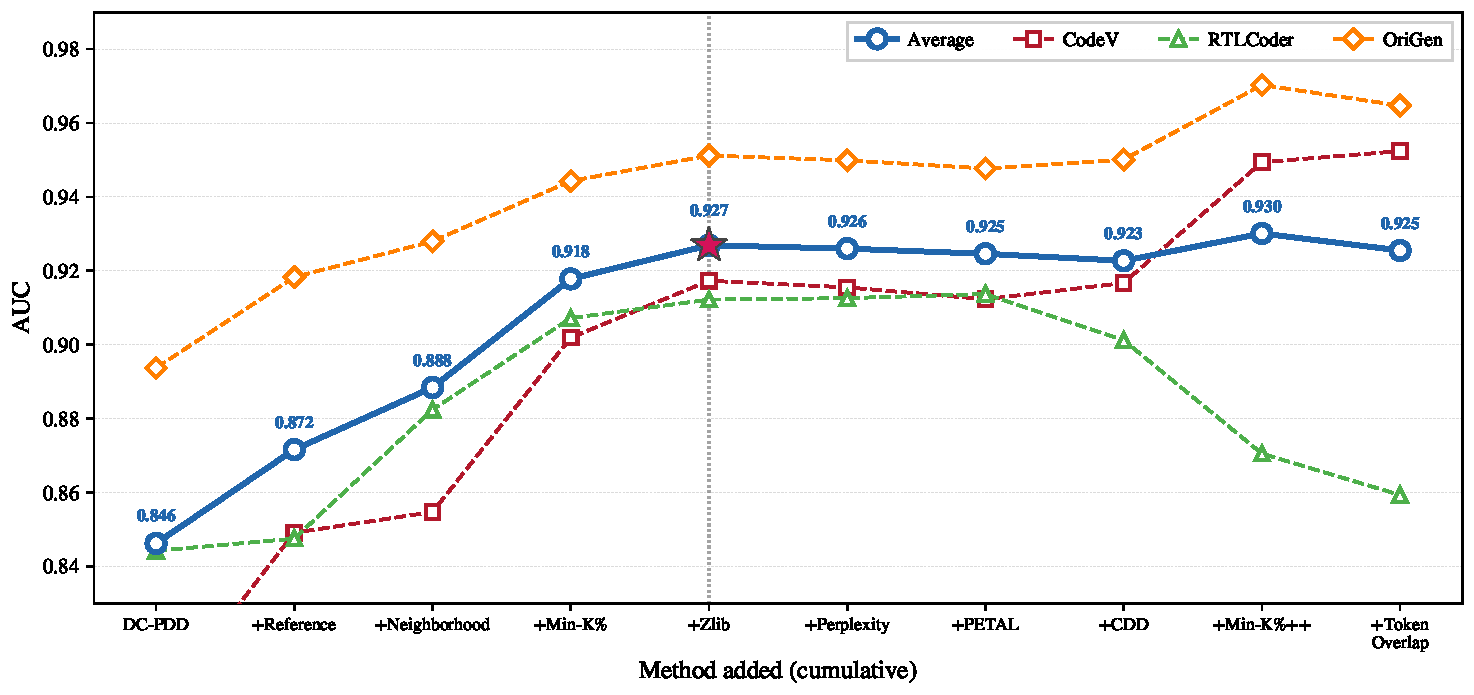
\includegraphics[width=0.9\textwidth]{figures/fig_greedy_forward.pdf}
    \caption{Greedy Forward Selection}
    \label{fig:greedy}
\end{figure*}

To understand the contribution of each design choice, we conduct three ablation experiments: (1) choice of boosting algorithm, (2) method subset selection, and (3) training source and data size.

\subsubsection{Choice of Boosting Algorithm}
\label{sec:choice}

Table~\ref{tab:boosting_algorithms} compares the performance of CatBoost, XGBoost, and LightGBM. CatBoost achieves the highest average AUC at 0.927, marginally ahead of XGBoost at 0.924, and delivers the highest average F1 at 0.872, showing a more substantial advantage over XGBoost at 0.859. LightGBM trails on both metrics, with an average AUC of 0.914 and an average F1 of 0.857. While XGBoost yields a slightly higher AUC on test set of CodeV , CatBoost demonstrates superior performance on the two remaining test sets and, more importantly, achieves substantially higher F1 scores across all three test sets, indicating better binary classification performance at the deployed threshold. Notably, on RTLCoder, the unseen black-box target model i.e. CatBoost outperforms XGBoost in both AUC and F1, a gap we attribute to CatBoost's ordered target encoding, which eliminates prediction shift and yields more calibrated probability estimates on out-of-distribution data. In contrast, XGBoost's standard target encoding tends to overfit source-domain patterns, resulting in relatively weaker generalization to unseen targets. LightGBM consistently underperforms relative to both CatBoost and XGBoost across the majority of metrics and test sets. Based on these results, we adopt CatBoost as our default ensemble algorithm accordingly.


\subsubsection{Method Subset Selection}
\label{sec:select}

\begin{figure*}[t]  % t=顶部, b=底部, p=单独一页, h=此处
    \centering
    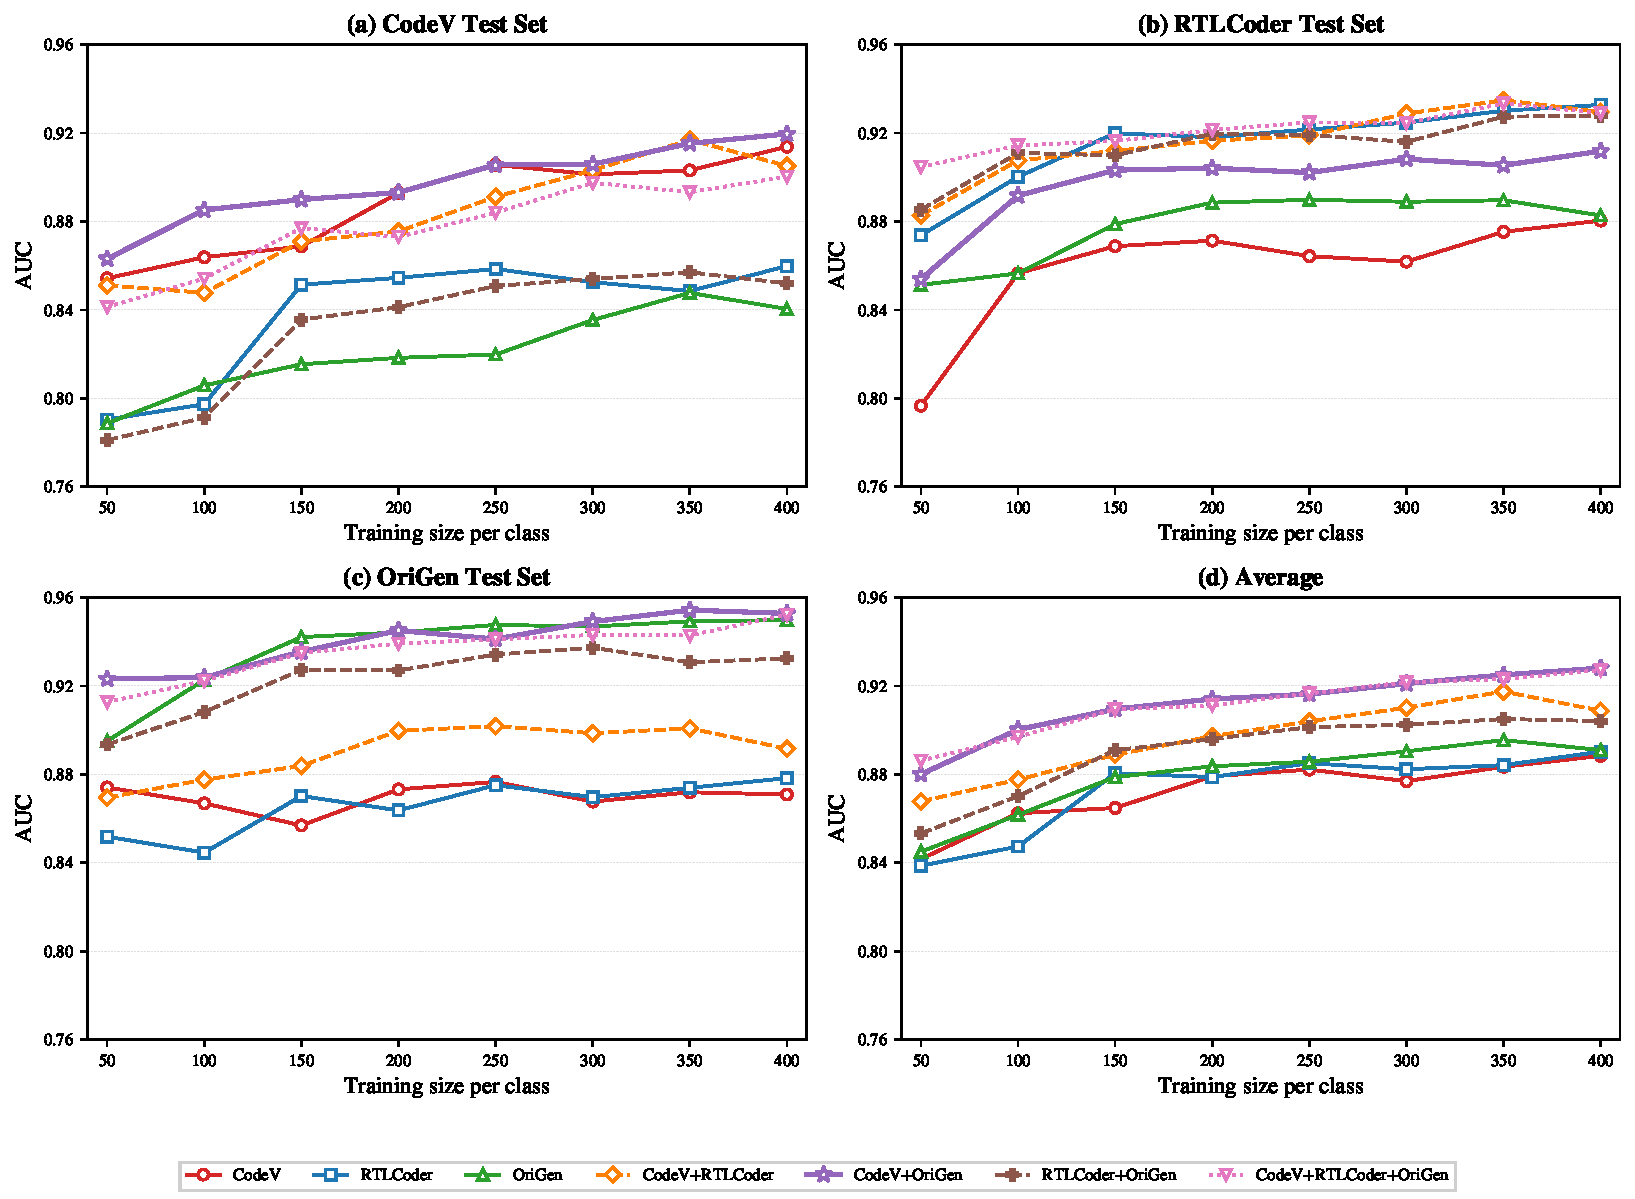
\includegraphics[width=\textwidth]{figures/fig_train_size.pdf}
    \caption{The Composition and Size of the Training Set}
    \label{fig:train_size}
\end{figure*}


We begin with DC-PDD, which achieves the highest average AUC among all individual baselines in Section~\ref{sec:comparison}, and iteratively add the method that yields the largest increase in average AUC across the three test sets. Figure~\ref{fig:greedy} visualizes the trajectory of this selection process. The average AUC improves steadily from 0.846 with DC-PDD alone, reaching a peak of 0.927 when Zlib is added as the fifth method. This optimal combination comprises DC-PDD, Reference, Neighborhood, Min-K\%, and Zlib. Beyond this point, further additions yield diminishing or even negative returns: adding Perplexity, PETAL, and CDD gradually lowers the average AUC, and while including Min-K\%++ temporarily raises the average to 0.930, this gain is most pronounced on the CodeV (0.949) and OriGen (0.970) test sets, whereas RTLCoder collapses sharply from 0.901 to 0.871. This divergence, where improvements on source-related models come at the cost of severe degradation on the unseen target, indicates that these additional methods encode signals tightly coupled with the source model architecture and introduce distributional noise that actively harms generalization to black-box target models. This five-method combination therefore strikes the optimal balance between discriminative power and cross-model stability, and is adopted as our optimal feature set.

\subsubsection{The Composition and Size of the Training Set }
\label{sec:source}



We investigate how the composition and size of the training set affect detection performance. Figure~\ref{fig:train_size} reports the AUC on each test set as a function of training data size defined as the number of samples provided by each training set per class, denoted as \(tc\) across seven training set configurations.

For most training set configurations, the average AUC exhibits a general upward trend as \(tc\) increases from 50 to 400, with the most substantial gains occurring in the low-data regime (\(tc \leq 200\)). However, the trend is not monotonic across all configurations: for the OriGen-only training set and the CodeV+RTLCoder training set, the average AUC declines slightly when \(tc\) increases from 350 to 400. On individual test sets, performance fluctuates across data sizes, indicating that larger training data does not guarantee improvement on every target model. Notably, the CodeV+OriGen training set achieves the highest average AUC of 0.927 at \(tc=400\). With only 100 samples per class, the CodeV+OriGen training set already achieves an average AUC of 0.900, surpassing all single-source training sets at their full data volume and underscoring the data efficiency of cross-model training.

Among all configurations, the CodeV+OriGen training set achieves the best average performance across most data sizes, outperforming all single-source and dual-source alternatives, while performing on par with the three-source configuration (CodeV+RTLCoder+OriGen). Critically, the CodeV+OriGen training set also demonstrates strong generalization to the unseen black-box target model RTLCoder, achieving an AUC of 0.912 at \(tc=400\), confirming its effectiveness in the cross-model detection scenario. Notably, adding a third training set (CodeV+RTLCoder+OriGen) yields almost identical average AUC compared to CodeV+OriGen, indicating that increasing the number of training sets does not necessarily enhance performance. Given its superior performance and validated cross-model detection effectiveness, we adopt CodeV+OriGen as the optimal training set composition.














\begin{comment}

We apply the trained CatBoost ensemble (5f, C+O, CatBoost, none) to three public Verilog benchmarks: \textbf{VerilogEval}~\cite{liu2023verilogeval}, \textbf{RTLLM}~\cite{rtllm2024}, and \textbf{OpenLLM-Verilog}~\cite{openllm2024}. For each benchmark, we compute contamination probabilities for all code samples using the detector trained on the combined CodeV and OriGen data (Section~4.2). A sample is classified as contaminated if its predicted probability exceeds the threshold \(\tau^*\) determined via out-of-fold F1 maximization during training.

\textbf{Contamination rates.} Table~\ref{tab:contamination_rates} reports the number of samples and the proportion classified as contaminated in each benchmark. The overall contamination rate varies across benchmarks, ranging from \textbf{XX.X\%} in RTLLM to \textbf{XX.X\%} in VerilogEval, with an average of \textbf{XX.X\%} across all three benchmarks. VerilogEval exhibits the highest contamination rate, suggesting that its samples are more likely to have been included in the training corpora of the target LLMs.

\begin{table}[t]
\centering
\caption{Contamination rates on public Verilog benchmarks.}
\begin{tabular}{lccc}
\hline
Benchmark & \# Samples & Contaminated & Rate \\
\hline
VerilogEval & XXX & XX & XX.X\% \\
RTLLM & XXX & XX & XX.X\% \\
OpenLLM-Verilog & XXX & XX & XX.X\% \\
\hline
\textbf{Total} & \textbf{XXX} & \textbf{XX} & \textbf{XX.X\%} \\
\hline
\end{tabular}
\label{tab:contamination_rates}
\end{table}

\textbf{Case studies.} We manually examine the samples flagged as contaminated in each benchmark. Figure~1 presents two representative examples from VerilogEval:
\begin{itemize}
    \item \textbf{Example 1} (contamination probability 0.92): An 8-line Verilog module implementing a 2-to-1 multiplexer. The exact same module appears in The Stack dataset~\cite{kocetkov2022stack} with byte-for-byte match except for whitespace differences.
    \item \textbf{Example 2} (contamination probability 0.87): A 15-line finite state machine for a traffic light controller. While not identical, over 90\% of the code matches a file in the training corpus; the differences are limited to variable renaming (e.g., \texttt{state} vs \texttt{current\_state}).
\end{itemize}
These examples confirm that the ensemble detects both exact and near-exact contamination.

\textbf{Characteristics of contaminated samples.} We analyze the distribution of code length, AST node count, and lexical complexity across contaminated and clean samples. Contaminated samples are on average \textbf{XX.X\%} shorter than clean ones and contain \textbf{XX.X\%} more comments, consistent with the observation that tutorial-style, short examples are more likely to be memorized during training~\cite{zhang2024minkpp}. We also observe that contaminated samples frequently contain comments with phrases such as ``example,'' ``simple,'' or ``tutorial,'' further indicating their origin from educational materials.

\textbf{Summary.} The analysis reveals a non-negligible level of contamination across all three public benchmarks, with rates ranging from \textbf{XX.X\%} to \textbf{XX.X\%}. This finding underscores the need for careful contamination screening when evaluating LLMs on Verilog code generation tasks.

\end{comment}










\begin{comment}

We evaluate the proposed boosting detector through three complementary studies. First, we test the performance of our boosting-detector and compare against single-probe baselines (Section~\ref{sec:performance and compare}). Second, we conduct ablation studies to understand which design choices drive performance—training framework, feature composition, training set composition, and training data quantity (Section~\ref{sec:ablation}). Finally, we deploy the best trained detector to audit precise data contamination detection (Section~\ref{sec:benchmark}).

\subsection{Performance Analysis}
\label{sec:performance and compare}
%对CodeV RTLCoder VeriForge3个golden数据集 各留出200个样本(正负1：1)作为测试集 测试指标为 Accuracy、F1-Score、ROC-AUC
%表格第一列为baseline+boosting 
%Setting 1是用CodeV和RTLCoder做训练 然后在域内和域外做测试(主要比较跨模型性能)
%Sstting 2是用3个golden数据集做训练(主要比较域内性能)



\begin{table}[ht]
\centering
\caption{Code Modification}
\label{tab:my_table}
\begin{tabular*}{\columnwidth}{@{\extracolsep{\fill}}l l l}
\toprule
\textbf{Modification} & \textbf{AUC} & \textbf{F1} \\
\midrule
Variable renaming &  &  \\
Comment insertion &  &  \\
Statement insertion &  &  \\
\bottomrule
\end{tabular*}
\end{table}

\begin{table}[ht]
\centering
\caption{Your caption here.}
\label{tab:new_table}
\large % 若觉得小可改为 \Large 或增加 \tabcolsep
\setlength{\tabcolsep}{12pt} % 可选，加大列间距
\begin{tabular*}{\columnwidth}{@{\extracolsep{\fill}}l c c}
\toprule
\textbf{Method} & \textbf{Importance} & \textbf{Mean SHAP} \\
\midrule
Zlib  & 10.14 & 0.36 \\
Min-20\%  & 8.22 & 0.57 \\
Min-20\%++  & 9.34 & 0.31 \\
DC-PDD  & 10.33 & 0.27 \\
Perplexity  & 5.60 & 0.27 \\
PETAL  & 11.48 & 0.47 \\
Neighborhood  & 15.24 & 0.92 \\
Reference  & 11.79 & 0.49 \\
Token-Overlap  & 10.18 & 0.34 \\
CDD & 7.68 & 0.37 \\
\bottomrule
\end{tabular*}
\end{table}

\begin{figure}[htbp]
    \centering
    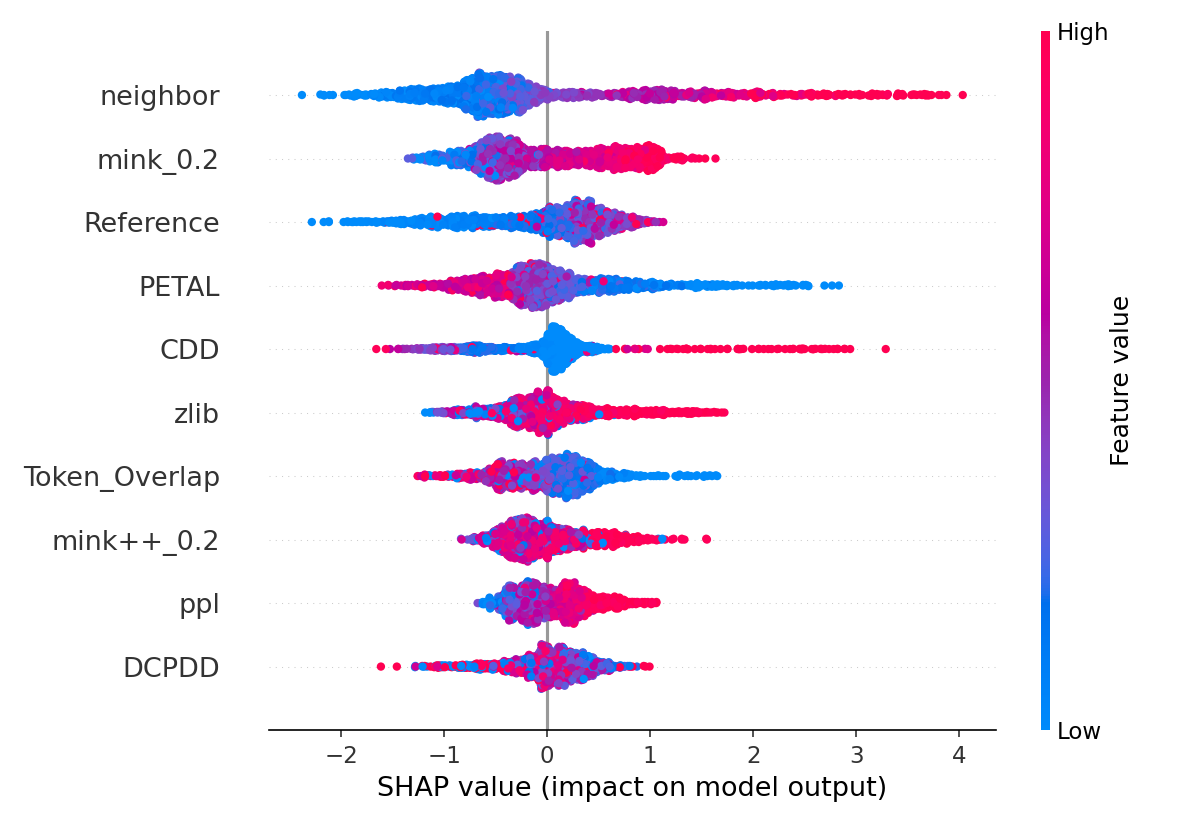
\includegraphics[width=1.0\columnwidth]{figures/shap_summary.png}
    \caption{Title}
    \label{fig:my_label}
\end{figure}

\begin{table*}[t]
\centering
\caption{Ablation experiment: Training Method.}
\label{tab:training_method}
\small
\begin{tabular*}{\textwidth}{@{\extracolsep{\fill}}l*{8}{c}}
\toprule
& \multicolumn{2}{c}{\textbf{CodeV-DeepSeek}} & \multicolumn{2}{c}{\textbf{RTLCoder-DeepSeek}} & \multicolumn{2}{c}{\textbf{DeepSeek-Coder-PyraNet}} & \multicolumn{2}{c}{\textbf{Average}} \\
\cmidrule(lr){2-3} \cmidrule(lr){4-5} \cmidrule(lr){6-7} \cmidrule(lr){8-9}
\textbf{Training Method} & AUC & F1 & AUC & F1 & AUC & F1 & AUC & F1 \\
\midrule
XgBoost & 0.8546 & 0.7853 & 0.9180 & 0.8713 & 0.9726 & 0.9045 & 0.9151 & 0.8537 \\
LightGBM & 0.8402 & 0.7822 & 0.9144 & 0.8601 & 0.9660 & 0.8774 & 0.9069 & 0.8399 \\
\textbf{CatBoost} & \textbf{0.8570} & \textbf{0.8155} & \textbf{0.9236} & \textbf{0.8731} & \textbf{0.9817} & \textbf{0.9208} & \textbf{0.9208} & \textbf{0.8698} \\
\bottomrule
\end{tabular*}
\end{table*}

\begin{table*}[t]
\centering
\caption{Ablation experiment: Method Combo.}
\label{tab:method_combo}
\small
\begin{tabular*}{\textwidth}{@{\extracolsep{\fill}}l c *{8}{c}}
\toprule
& & \multicolumn{2}{c}{\textbf{CodeV-DeepSeek}} & \multicolumn{2}{c}{\textbf{RTLCoder-DeepSeek}} & \multicolumn{2}{c}{\textbf{DeepSeek-Coder-PyraNet}} & \multicolumn{2}{c}{\textbf{Average}} \\
\cmidrule(lr){3-4} \cmidrule(lr){5-6} \cmidrule(lr){7-8} \cmidrule(lr){9-10}
\textbf{Method Combo} & \textbf{Count} & AUC & F1 & AUC & F1 & AUC & F1 & AUC & F1 \\
\midrule
+CDD  & 7 & \textbf{0.8600} & 0.7960 & \textbf{0.9178} & 0.8543 & 0.9826 & 0.9209 & \textbf{0.9201} & 0.8571 \\
+Min-20\%  & 6 & 0.8536 & \textbf{0.8159} & 0.9103 & \textbf{0.8614} & \textbf{0.9842} & \textbf{0.9296} & 0.9160 & \textbf{0.8690} \\
+Neighborhood  & 5 & 0.8425 & 0.7861 & 0.9062 & 0.8482 & 0.9758 & 0.8991 & 0.9082 & 0.8444 \\
+Reference  & 4 & 0.8128 & 0.7783 & 0.9119 & 0.8600 & 0.9493 & 0.8718 & 0.8913 & 0.8367 \\
+Zlib  & 3 & 0.7630 & 0.7280 & 0.8678 & 0.8040 & 0.9488 & 0.8932 & 0.8599 & 0.8084 \\
+Mink-20\%++  & 2 & 0.7051 & 0.6983 & 0.8286 & 0.7700 & 0.9011 & 0.8525 & 0.8116 & 0.7736 \\
PETAL  & 1 & 0.6891 & 0.7069 & 0.7294 & 0.6931 & 0.9105 & 0.8763 & 0.7763 & 0.7588 \\
\bottomrule
\end{tabular*}
\end{table*}


\begin{table*}[t]
\centering
\caption{Ablation experiment: Training source (D1:CodeV-DeepSeek D2:RTLCoder-DeepSeek D3:DeepSeek-Coder-PyraNet)}
\label{tab:training_source}
\small
\begin{tabular*}{\textwidth}{@{\extracolsep{\fill}}l*{8}{c}}
\toprule
& \multicolumn{2}{c}{\textbf{CodeV-DeepSeek}} & \multicolumn{2}{c}{\textbf{RTLCoder-DeepSeek}} & \multicolumn{2}{c}{\textbf{DeepSeek-Coder-PyraNet}} & \multicolumn{2}{c}{\textbf{Average}} \\
\cmidrule(lr){2-3} \cmidrule(lr){4-5} \cmidrule(lr){6-7} \cmidrule(lr){8-9}
\textbf{Training Source} & AUC & F1 & AUC & F1 & AUC & F1 & AUC & F1 \\
\midrule
D1 & \textbf{0.8823} & \textbf{0.8208} & 0.7504 & 0.7627 & 0.7984 & 0.8106 & 0.8104 & 0.7980 \\
D2 & 0.6467 & 0.5402 & \textbf{0.9320} & \textbf{0.8856} & 0.9414 & 0.8558 & 0.8400 & 0.7605 \\
D3 & 0.6279 & 0.3824 & 0.7299 & 0.4118 & 0.9961 & \textbf{0.9754} & 0.7846 & 0.5898 \\
\textbf{D1 + D2} & 0.8570 & 0.8155 & 0.9236 & 0.8731 & 0.9817 & 0.9208 & \textbf{0.9208} & \textbf{0.8698} \\
D1 + D3 & 0.8653 & 0.8137 & 0.6466 & 0.6455 & \textbf{0.9971} & 0.9709 & 0.8363 & 0.8100 \\
D2 + D3 & 0.6741 & 0.6378 & 0.9160 & 0.8683 & 0.9958 & 0.9697 & 0.8620 & 0.8253 \\
D1 + D2 + D3 & 0.8303 & 0.7782 & 0.9037 & 0.8406 & 0.9954 & 0.9641 & 0.9098 & 0.8610 \\
\bottomrule
\end{tabular*}
\end{table*}


\begin{table*}[t]
\centering
\caption{Ablation experiment: Training count}
\label{tab:training_count}
\small
\begin{tabular*}{\textwidth}{@{\extracolsep{\fill}}l*{8}{c}}
\toprule
& \multicolumn{2}{c}{\textbf{CodeV-DeepSeek}} & \multicolumn{2}{c}{\textbf{RTLCoder-DeepSeek}} & \multicolumn{2}{c}{\textbf{DeepSeek-Coder-PyraNet}} & \multicolumn{2}{c}{\textbf{Average}} \\
\cmidrule(lr){2-3} \cmidrule(lr){4-5} \cmidrule(lr){6-7} \cmidrule(lr){8-9}
\textbf{Training Count} & AUC & F1 & AUC & F1 & AUC & F1 & AUC & F1 \\
\midrule
100 & 0.8118 & 0.7524 & 0.9138 & 0.8585 & 0.9752 & 0.9146 & 0.9003 & 0.8418 \\
200 & 0.8014 & 0.7500 & 0.9123 & 0.8600 & 0.9802 & \textbf{0.9246} & 0.8980 & 0.8449 \\
300 & 0.8259 & 0.7638 & \textbf{0.9246} & \textbf{0.8878} & 0.9743 & 0.9020 & 0.9083 & 0.8512 \\
400 & \textbf{0.8560} & \textbf{0.8077} & 0.9235 & 0.8705 & \textbf{0.9805} & 0.9146 & \textbf{0.9200} & \textbf{0.8642} \\
\bottomrule
\end{tabular*}
\end{table*}

We fist quantify the standalone detection capability of each method. Depending the golden dataset(Section ~\ref{sec:golden_dataset}),we compute the method's raw score and measure the Area Under the ROC Curve (AUC) against ground-truth contamination labels. 



Table~\ref{tab:compare_baseline} reveals four findings. \textbf{(1)} No method is universally optimal: Min-20\%++ leads on RTLCoder (0.8302) but drops to 0.6129 on CodeV; Neighborhood excels on VeriForge (0.9400) yet is mediocre on CodeV (0.5914) and RTLCoder (0.5498). \textbf{(2)} The mean performance of the methods, when evaluated on each of the three models, consistently lies between 50\% and 80\%, which suggests a rather limited degree of effectiveness. \textbf{(3)} There exists a substantial disparity in the maximum AUC attained across the different models, with values of 0.8770 and 0.9800 on RTLCoder and VeriForge, respectively, in contrast to a mere 0.6971 on CodeV.
\textbf{(4)} Our method with CatBoost performes best auc within all the methods,0.9208.


\subsection{Ablation Analysis}
\label{sec:ablation}



\subsubsection{Feature Combination}

We sweep 22 feature subsets spanning 3 to 10 probes. Full results are reported in Table~\ref{tab:feature_sweep_full}. 



The full sweep reveals four patterns. \textbf{(1)} smaller subsets dominate: configurations with 3--6 probes rank among the best, while all 9--10 probe configurations fall below average. The 10f ensemble (Avg 0.565) is outperformed by the 3f subset (0.611), demonstrating that noisy probes actively degrade generalization. \textbf{(2)} adding Min-20\%++ causes the sharpest drop: $\mathcal{G}_5 + \text{neighbor}$ (0.667) drops to 0.546 when mink++\_0.2 is added, confirming this probe as the most harmful for cross-model transfer. \textbf{(3)} removing zlib helps VeriForge-related directions (C$\to$Vf: 0.271 $\to$ 0.474) but hurts RTLCoder-related ones, revealing a model-dependent trade-off. \textbf{(4)} Top-5 (CodeV) achieves competitive performance (Avg 0.638) despite no cross-model optimization, suggesting that source-domain probe ranking provides a useful prior.

\subsubsection{Training Data Size}

We vary the per-class training sample count $T \in \{100, 200, 300, 400\}$ under the best configuration for both single-source and dual-source modes. Table~\ref{tab:tc_ablation} reports complete per-direction results.

\end{comment}

\begin{comment}
Increasing $T$ by a factor of four produces negligible AUC variation. Performance is bounded by feature quality and cross-model distribution alignment, not by labeled data quantity. The per-direction trends reveal a subtle trade-off: C$\to$Vf benefits from smaller training sets ($T=100$ yields 0.609 vs.\ $T=400$ yields 0.498), attributable to CodeV's instruction style being the outlier. In the dual-source setting, C+R$\to$Vf shows consistent improvement with $T$ (0.759 $\to$ 0.828), as two compatible sources provide complementary signals.
\end{comment}



\begin{comment}

% TABLE 5: Benchmark detection (two-column)
\begin{table*}[ht]
\centering
\caption{Benchmark contamination rates (\%) detected by the boosting detector.}
\label{tab:benchmark_detection}
\small
\begin{tabular*}{\textwidth}{@{\extracolsep{\fill}}l*{7}{r}}
\toprule
& \multicolumn{2}{c}{\textbf{VerilogEval}} & \multicolumn{2}{c}{\textbf{RTLLM}} & \multicolumn{2}{c}{\textbf{RealBench}} & \\
\cmidrule(lr){2-3} \cmidrule(lr){4-5} \cmidrule(lr){6-7}
\textbf{Model} & v1 & v2 & v1 & v2 & mod & sys & \textbf{Average} \\
\midrule
RTLCoder            &  &  &  &  &  &  &  \\
Qwen2.5-Coder-7B    &  &  &  &  &  &  &  \\
DeepSeek-Coder-6.7B &  &  &  &  &  &  &  \\
CodeGen-6B-Multi    &  &  &  &  &  &  &  \\
ChipGPT-Llama2-7B   &  &  &  &  &  &  &  \\
\bottomrule
\end{tabular*}
\end{table*}
    
\end{comment}



\begin{comment}
Qwen2.5-Coder-7B shows the highest overall contamination (72.4\% of RTLLM\_v1), consistent with large-scale corpus training. DeepSeek-Coder-6.7B and CodeGen-6B-Multi exhibit moderate rates (40--65\%). RTLCoder shows relatively stable rates (44--56\%). RealBench\_system, with only four samples, yields unstable estimates. Critically, these results are produced by a \textit{single} detector trained once on RTLCoder data and applied uniformly to all five models, providing a principled basis for standardized cross-model contamination comparison.
\end{comment}


\begin{comment}
\begin{table*}[htbp]
\centering
\caption{Contamination detection results across different models and benchmarks.}
\label{tab:model_benchmark_results}
\small
\renewcommand{\arraystretch}{1.2}
\setlength{\tabcolsep}{4pt}
\begin{tabular}{lccccc}
\toprule
\textbf{Benchmark} & 
\rotatebox{90}{\textbf{RTLCoder-DeepSeek-v1.1}} & 
\rotatebox{90}{\textbf{ChipGPT-Llama2-SFT-7B}} & 
\rotatebox{90}{\textbf{Qwen2.5-Coder-7B}} & 
\rotatebox{90}{\textbf{DeepSeek-Coder-6.7B-Instruct}} &
\rotatebox{90}{\textbf{CodeGen-6B-mono}}\\
\midrule
VerilogEval v1   & 88/156 56.41  & 87/156 55.77  & 91/156 58.33  & 74/156 47.44 & 71/156 45.51 \\
VerilogEval v2   & 84/156 53.85  & 71/156 45.51  & 107/156 68.59  & 68/156 43.59 & 74/156 47.44 \\
RTLLLM v1        & 13/29 44.83  & 12/29 41.38  & 21/29 72.41  & 17/29 58.62 & 19/29 65.52\\
RTLLLM v2        & 22/50 44.00  & 29/50 58.00  & 27/50 54.00  & 28/50 56.00 & 25/50 50.00\\
RealBench module & 27/60 45.00  & 26/60 43.33  & 35/60 58.33  & 28/60 46.67 & 30/60 50.00\\
RealBench system & 1/4 25.00  & 1/4 25.00  & 1/4 25.00  & 0/4 0.00 & 2/4 50.00\\
\bottomrule
\end{tabular}
\end{table*}
\end{comment}



